\documentclass{article}
\usepackage{endfloat}
\usepackage{graphicx}

\makeatletter
\efloat@openpost{fff}
\efloat@iwrite{fff}{\string\textwidth=\the\textwidth}% pass \textwidth to fff file
\makeatother

\begin{document}

\begin{figure}
    \centering
    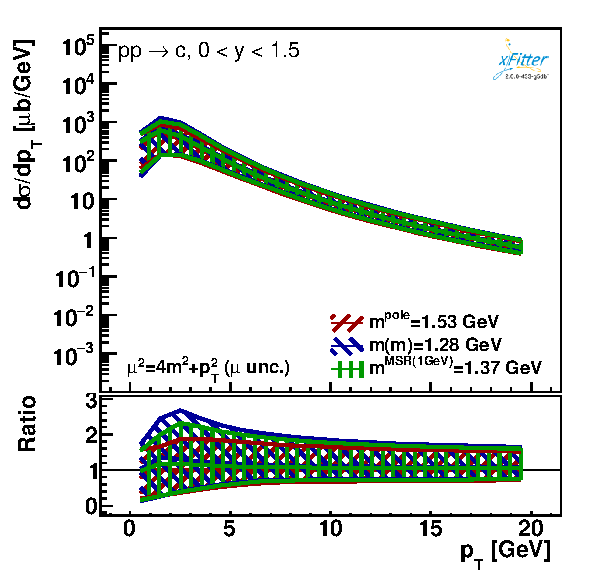
\includegraphics[width=0.49\textwidth]{figs/parton-ptmax20/dyn-therr3/data_401-1.pdf}
    \put(-169,-35){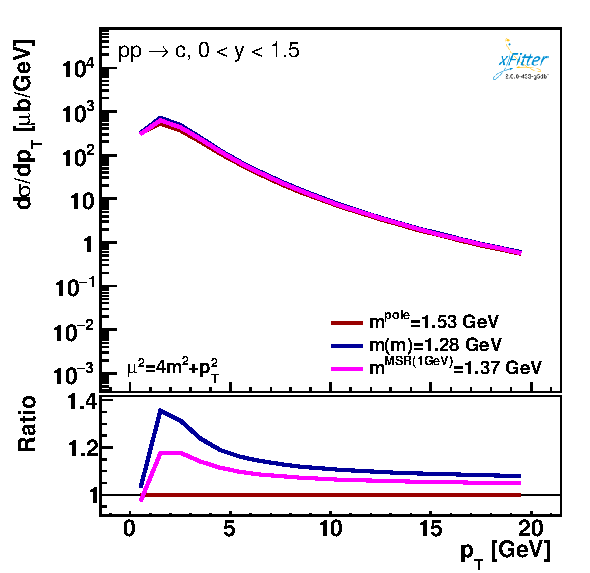
\includegraphics[width=0.49\textwidth,trim=0 0 0 190,clip=true]{figs/parton-ptmax20/dyn-therr3-onlynom/data_401-1.pdf}}
    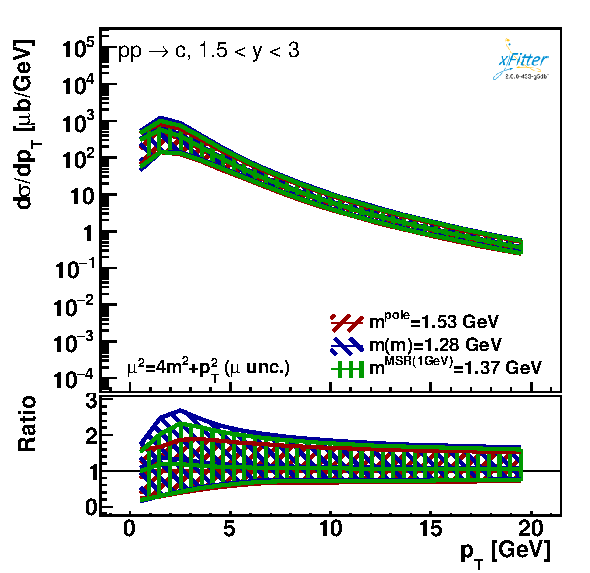
\includegraphics[width=0.49\textwidth]{figs/parton-ptmax20/dyn-therr3/data_401-2.pdf}
    \put(-169,-35){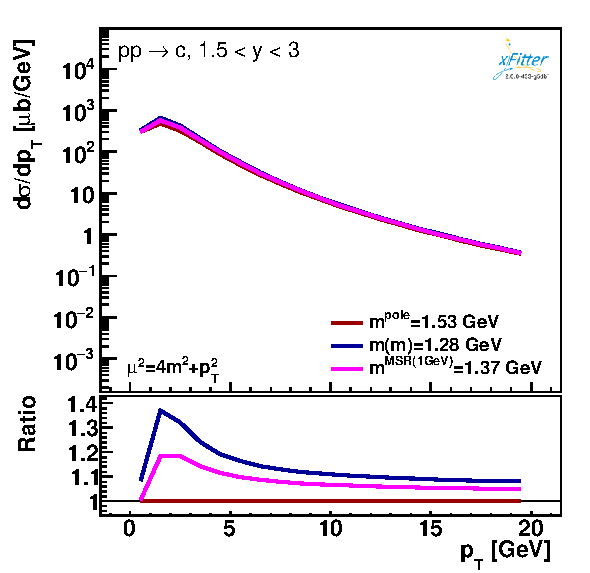
\includegraphics[width=0.49\textwidth,trim=0 0 0 190,clip=true]{figs/parton-ptmax20/dyn-therr3-onlynom/data_401-2.pdf}}\\
    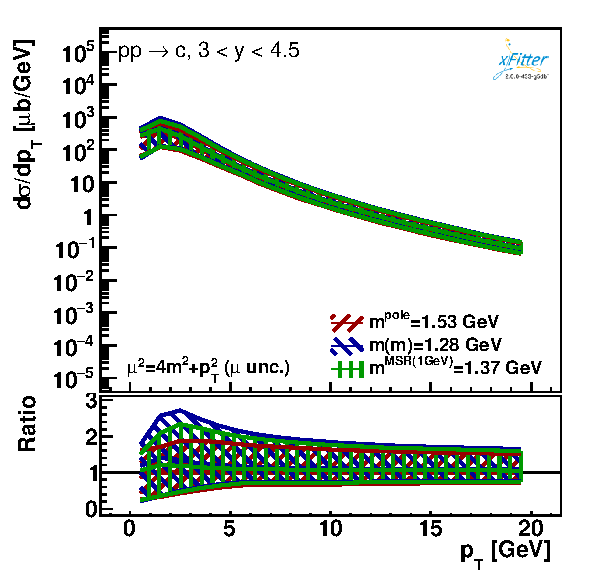
\includegraphics[width=0.49\textwidth]{figs/parton-ptmax20/dyn-therr3/data_401-3.pdf}
    \put(-169,-35){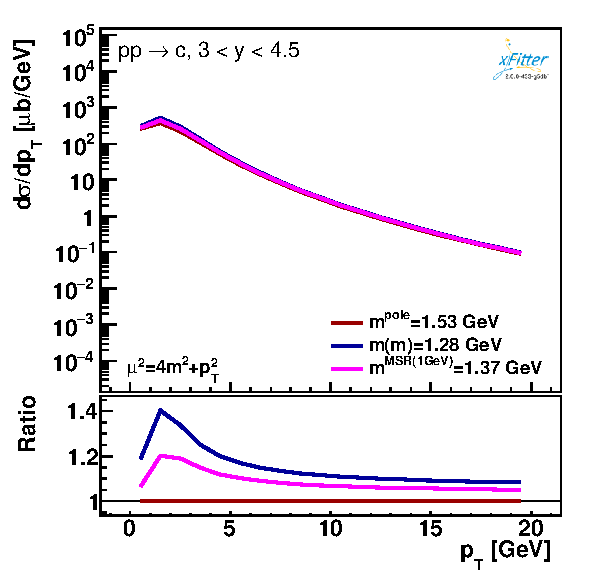
\includegraphics[width=0.49\textwidth,trim=0 0 0 190,clip=true]{figs/parton-ptmax20/dyn-therr3-onlynom/data_401-3.pdf}}
    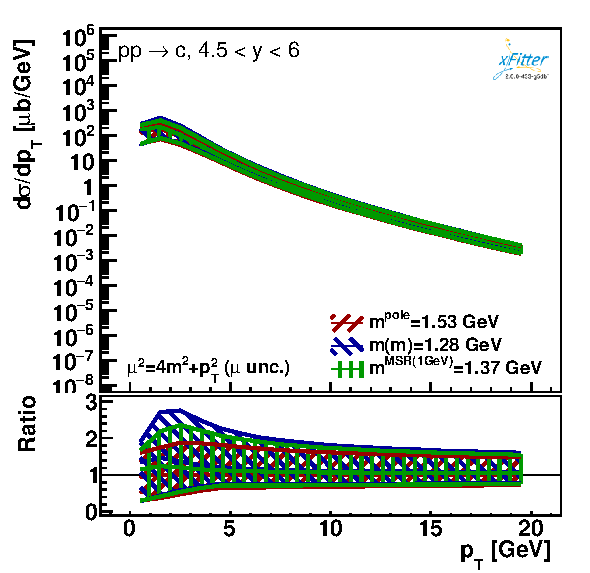
\includegraphics[width=0.49\textwidth]{figs/parton-ptmax20/dyn-therr3/data_401-4.pdf}
    \put(-169,-35){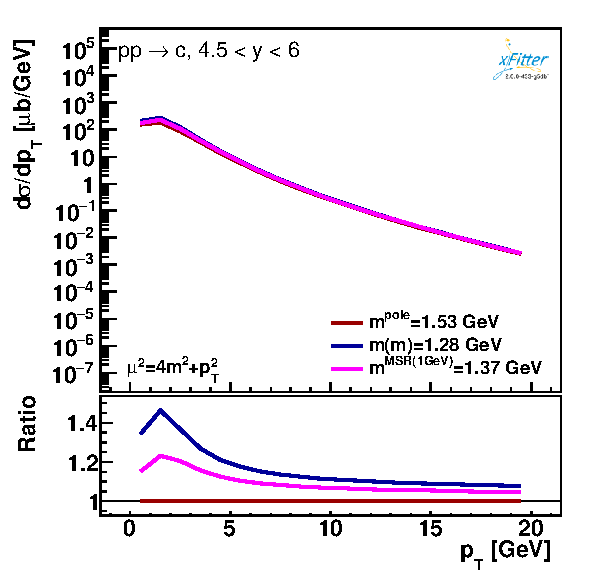
\includegraphics[width=0.49\textwidth,trim=0 0 0 190,clip=true]{figs/parton-ptmax20/dyn-therr3-onlynom/data_401-4.pdf}}
    \caption{}
    \label{fig:c-pty-mu}
\end{figure}

\end{document}
